

CDF of $X$, 
\begin{align}
    F(x) &=  \int_{-\infty}^xf(t)dt \\
    &= \int_{0}^xf(t)dt \hspace{1cm} \text{as } x>0\\
    &= \int_{-\infty}^t\left((\alpha t^{\alpha -1} + \beta t^{\beta-1} ) \times e^{-t^{\alpha}-t^{\beta}}\right)dt \\
    &= -e^{-t^{\alpha}-t^{\beta}} \Big|_0^x\\
    &= 1-e^{-x^{\alpha}-x^{\beta}}
\end{align}
Hazard function,
\begin{align}
    h(x) &= \frac{f(x)}{1-F(x)} \\
    &= \alpha x^{\alpha -1} + \beta x^{\beta-1} \\
    h^{\prime}(x) &= \alpha(\alpha -1) x^{\alpha -2} + \beta(\beta-1) x^{\beta-2}\\
     h^{\prime}(x) &= 
         \begin{cases}
    0 & \alpha=\beta=1 \\
    >0 & \text{otherwise}\\
    \end{cases}
    \end{align}
    Thus $h(x)$ can be either constant function or an increasing function.
    
    \begin{figure}[h]
    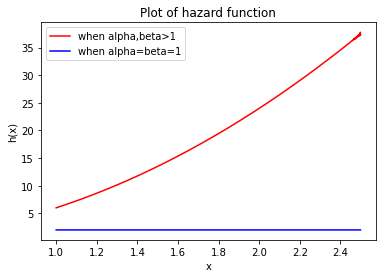
\includegraphics[width=\columnwidth]{solutions/2018/dec/118/figures/plot.png}
    \end{figure}
     From the above figure, it is verified that $h(x)$ can be either constant function or an increasing function.\\
       Correct options are 1,3.




